%%%%%%%%%%%%%%%%%%%%%%%%%%%%%%%%%%%%%%%%%
% Beamer Presentation
% LaTeX Template
% Version 1.0 (10/11/12)
%
% This template has been downloaded from:
% http://www.LaTeXTemplates.com
%
% License:
% CC BY-NC-SA 3.0 (http://creativecommons.org/licenses/by-nc-sa/3.0/)
%
%%%%%%%%%%%%%%%%%%%%%%%%%%%%%%%%%%%%%%%%%

%----------------------------------------------------------------------------------------
%	PACKAGES AND THEMES
%----------------------------------------------------------------------------------------

\documentclass[UTF8,aspectratio=169,14pt]{ctexbeamer}

\usepackage{hyperref}
\hypersetup{
	colorlinks=true,
	linkcolor=red,
	anchorcolor=blue,
	citecolor=green
}

\mode<presentation> {
	
	% The Beamer class comes with a number of default slide themes
	% which change the colors and layouts of slides. Below this is a list
	% of all the themes, uncomment each in turn to see what they look like.
	
	%\usetheme{default}
	%\usetheme{AnnArbor}
	%\usetheme{Antibes}
	%\usetheme{Bergen}
	%\usetheme{Berkeley}
	%\usetheme{Berlin}
	%\usetheme{Boadilla}
	%\usetheme{CambridgeUS}
	%\usetheme{Copenhagen}
	%\usetheme{Darmstadt}
	%\usetheme{Dresden}
	%\usetheme{Frankfurt}
	%\usetheme{Goettingen}
	%\usetheme{Hannover}
	%\usetheme{Ilmenau}
	%\usetheme{JuanLesPins}
	%\usetheme{Luebeck}
	\usetheme{Madrid}
	%\usetheme{Malmoe}
	%\usetheme{Marburg}
	%\usetheme{Montpellier}
	%\usetheme{PaloAlto}
	%\usetheme{Pittsburgh}
	%\usetheme{Rochester}
	%\usetheme{Singapore}
	%\usetheme{Szeged}
	%\usetheme{Warsaw}
	
	% As well as themes, the Beamer class has a number of color themes
	% for any slide theme. Uncomment each of these in turn to see how it
	% changes the colors of your current slide theme.
	
	%\usecolortheme{albatross}
	%\usecolortheme{beaver}
	%\usecolortheme{beetle}
	%\usecolortheme{crane}
	%\usecolortheme{dolphin}
	%\usecolortheme{dove}
	%\usecolortheme{fly}
	%\usecolortheme{lily}
	%\usecolortheme{orchid}
	%\usecolortheme{rose}
	%\usecolortheme{seagull}
	%\usecolortheme{seahorse}
	%\usecolortheme{whale}
	%\usecolortheme{wolverine}
	
	%\setbeamertemplate{footline} % To remove the footer line in all slides uncomment this line
	%\setbeamertemplate{footline}[page number] % To replace the footer line in all slides with a simple slide count uncomment this line
	
	%\setbeamertemplate{navigation symbols}{} % To remove the navigation symbols from the bottom of all slides uncomment this line
}

\usepackage{graphicx} % Allows including images
\graphicspath{{./figs/}}
\usepackage{booktabs} % Allows the use of \toprule, \midrule and \bottomrule in tables
\usepackage{longtable}
\usepackage{listings}
\usepackage{xcolor}
\lstset{numbers=left, %设置行号位置
	numberstyle=\tiny, %设置行号大小
	keywordstyle=\color{blue}, %设置关键字颜色
	commentstyle=\color[cmyk]{1,0,1,0}, %设置注释颜色
	frame=single, %设置边框格式
	escapeinside=``, %逃逸字符(1左面的键),用于显示中文
	%breaklines, %自动折行
	extendedchars=false, %解决代码跨页时,章节标题,页眉等汉字不显示的问题
	xleftmargin=2em,xrightmargin=2em, aboveskip=1em, %设置边距
	tabsize=4, %设置tab空格数
	showspaces=false %不显示空格
}
% Fonts
% \usepackage{libertine}
% \setmonofont{Courier}
\setCJKsansfont[ItalicFont=Noto Serif CJK SC Black, BoldFont=Noto Sans CJK SC Black]{Noto Sans CJK SC}


%----------------------------------------------------------------------------------------
%	TITLE PAGE
%----------------------------------------------------------------------------------------

\title[第1讲]{第1讲 :操作系统概述} % The short title appears at the bottom of every slide, the full title is only on the title page
\subtitle{第四节:为什么要学习和如何学习操作系统}
\author{向勇、陈渝、李国良} % Your name
\institute[清华大学] % Your institution as it will appear on the bottom of every slide, may be shorthand to save space
{
清华大学计算机系 \\ % Your institution for the title page
\medskip
\textit{xyong,yuchen,liguoliang@tsinghua.edu.cn} % Your email address
}
\date{\today} % Date, can be changed to a custom date

\begin{document}

\begin{frame}
\titlepage % Print the title page as the first slide
\end{frame}

%\begin{frame}
%\frametitle{提纲} % Table of contents slide, comment this block out to remove it
%\tableofcontents % Throughout your presentation, if you choose to use \section{} and \subsection{} commands, these will automatically be printed on this slide as an overview of your presentation
%\end{frame}
%
%%----------------------------------------------------------------------------------------
%%	PRESENTATION SLIDES
%%-----------------------------------------------\-----------------------------------------
%
%%------------------------------------------------
%\section{第四节:为什么要学习和如何学习操作系统} % Sections can be created in order to organize your presentation into discrete blocks, all sections and subsections are automatically printed in the table of contents as an overview of the talk
%%----------------------------------------------------------------------------------------

%------------------------------------------------
\begin{frame}
    \frametitle{操作系统课是多门课程的综合}
    
        \begin{columns}
    	
    	
    	\begin{column}{0.4\textwidth}	
    		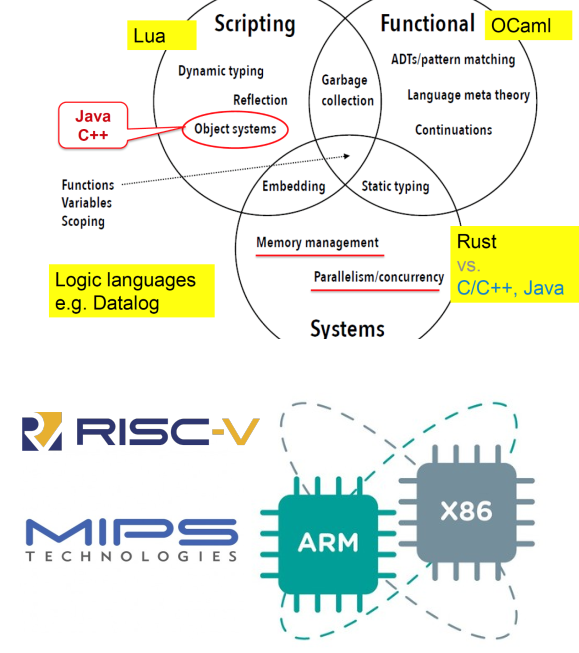
\includegraphics[width=1\linewidth]{lang-arch-os-relation}	
    	\end{column}
    	
    	\begin{column}{0.5\textwidth}
    		
    \begin{itemize}

        \item 综合课程-结合许多不同的课程
        \begin{itemize}
            \item 程序设计语言
            \item 数据结构
            \item 计算机组成原理/体系结构
            \item 编译技术
        \end{itemize} \pause
        \item OS基本理论基础
    	\begin{itemize}
    		\item 操作系统概念和原理
    	\end{itemize} \pause
        \item OS设计和实现
        \begin{itemize}
            \item 操作系统源代码\&实践技能
        \end{itemize}
    \end{itemize}

     \end{column}
\end{columns}

\end{frame}
    
\begin{frame}
    \frametitle{操作系统软件的地位}
    
            \begin{columns}
    	
    	
    	\begin{column}{0.35\textwidth}	
    		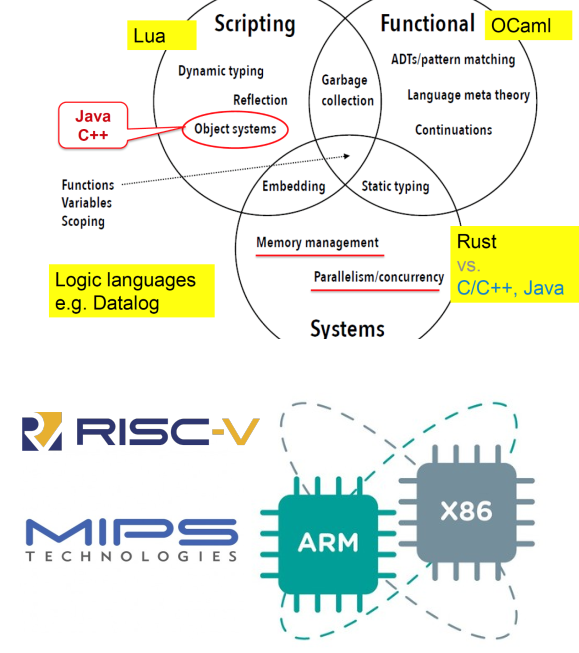
\includegraphics[width=1\linewidth]{lang-arch-os-relation}	
    	\end{column}
    	
    	\begin{column}{0.65\textwidth}
    		
        操作系统:计算机科学研究的基石之一
        \pause
        \begin{itemize}
            \item 计算机系统的基本组成部分和核心支撑软件
            \item 贯穿程序语言、运行时系统、应用、体系结构
            \item 联系计算机科学和计算机系统的典范 \pause 
            \item 操作系统的知识影响到专业人员的素质
            \item 大量专业工作与操作系统技术相关
        \end{itemize}

         \end{column}
\end{columns}

\end{frame}
%------------------------------------------------
\begin{frame}[plain]
    \frametitle{操作系统研究相关的图灵奖}
    \centering
     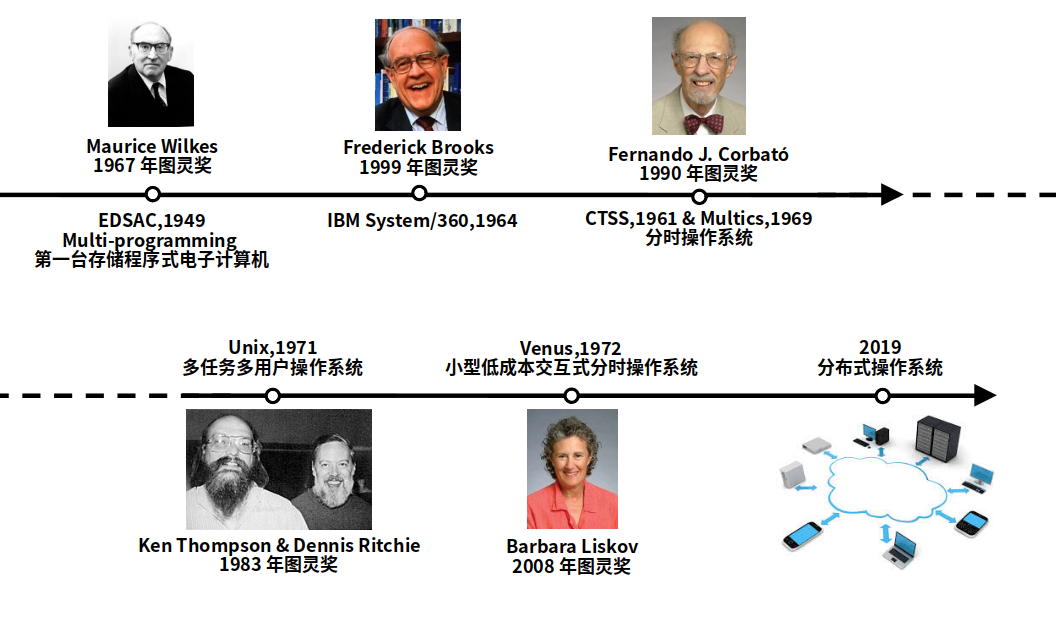
\includegraphics[width=0.8\linewidth]{turing-os}
     \\
     from sjtu os course
     %sjtu os course 
%http://www-31.ibm.com/ibm/cn/ibm100/icons/system360/index.shtml
%https://blog.csdn.net/deep_explore/article/details/6930582
%https://zhuanlan.zhihu.com/p/59664012 https://tech.ifeng.com/c/7oXlxnl6R5f
%https://kb.cnblogs.com/page/79904/
\end{frame}

\begin{frame}
    \frametitle{操作系统研究相关的产业}
     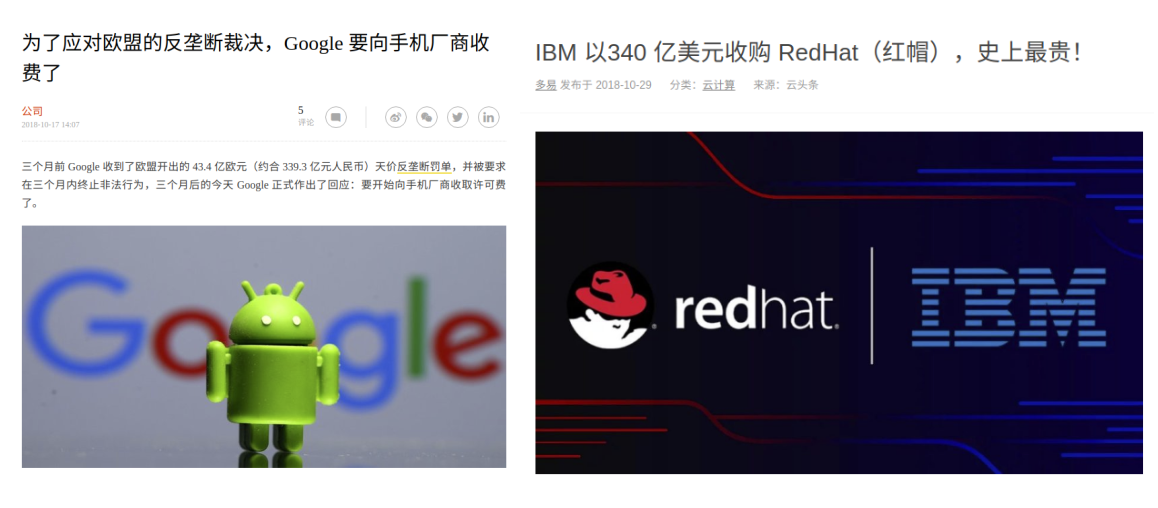
\includegraphics[width=1.0\linewidth]{companies-os}
     %sjtu os course 
\end{frame}

%------------------------------------------------
    
\begin{frame}
    \frametitle{哪里在做操作系统研究?}
    \begin{itemize}
%    	\pause
        \item 顶尖大学的计算机科学部门
         \begin{itemize}
        	\item MIT, Stanford, Berkeley, ...
         \end{itemize} \pause
        \item 计算机产业
        \begin{itemize}
            \item 旧时:Xerox (PARC), IBM, DEC (SRC), Bell Labs
            \item 现代:Microsoft, Google, Yahoo, IBM, HP, Sun, Intel, VMware, Amazon,  …
            \item 国内:华为、阿里巴巴、腾讯 …
        \end{itemize}\pause

        \item 学术研究协会
        \begin{itemize}
            \item SOSP OSDI HotOS
            \item ACM SIGOPS \href{http://www.sigops.org/award-hof.html}{Hall-of-Fame Awards} 
            \item USENIX USENIX-ATC
        \end{itemize}
    \end{itemize}
\end{frame}



%------------------------------------------------

\begin{frame}
    \frametitle{学习操作系统的目的}
    \begin{columns}
    	
    	
   \begin{column}{0.5\textwidth}	
   	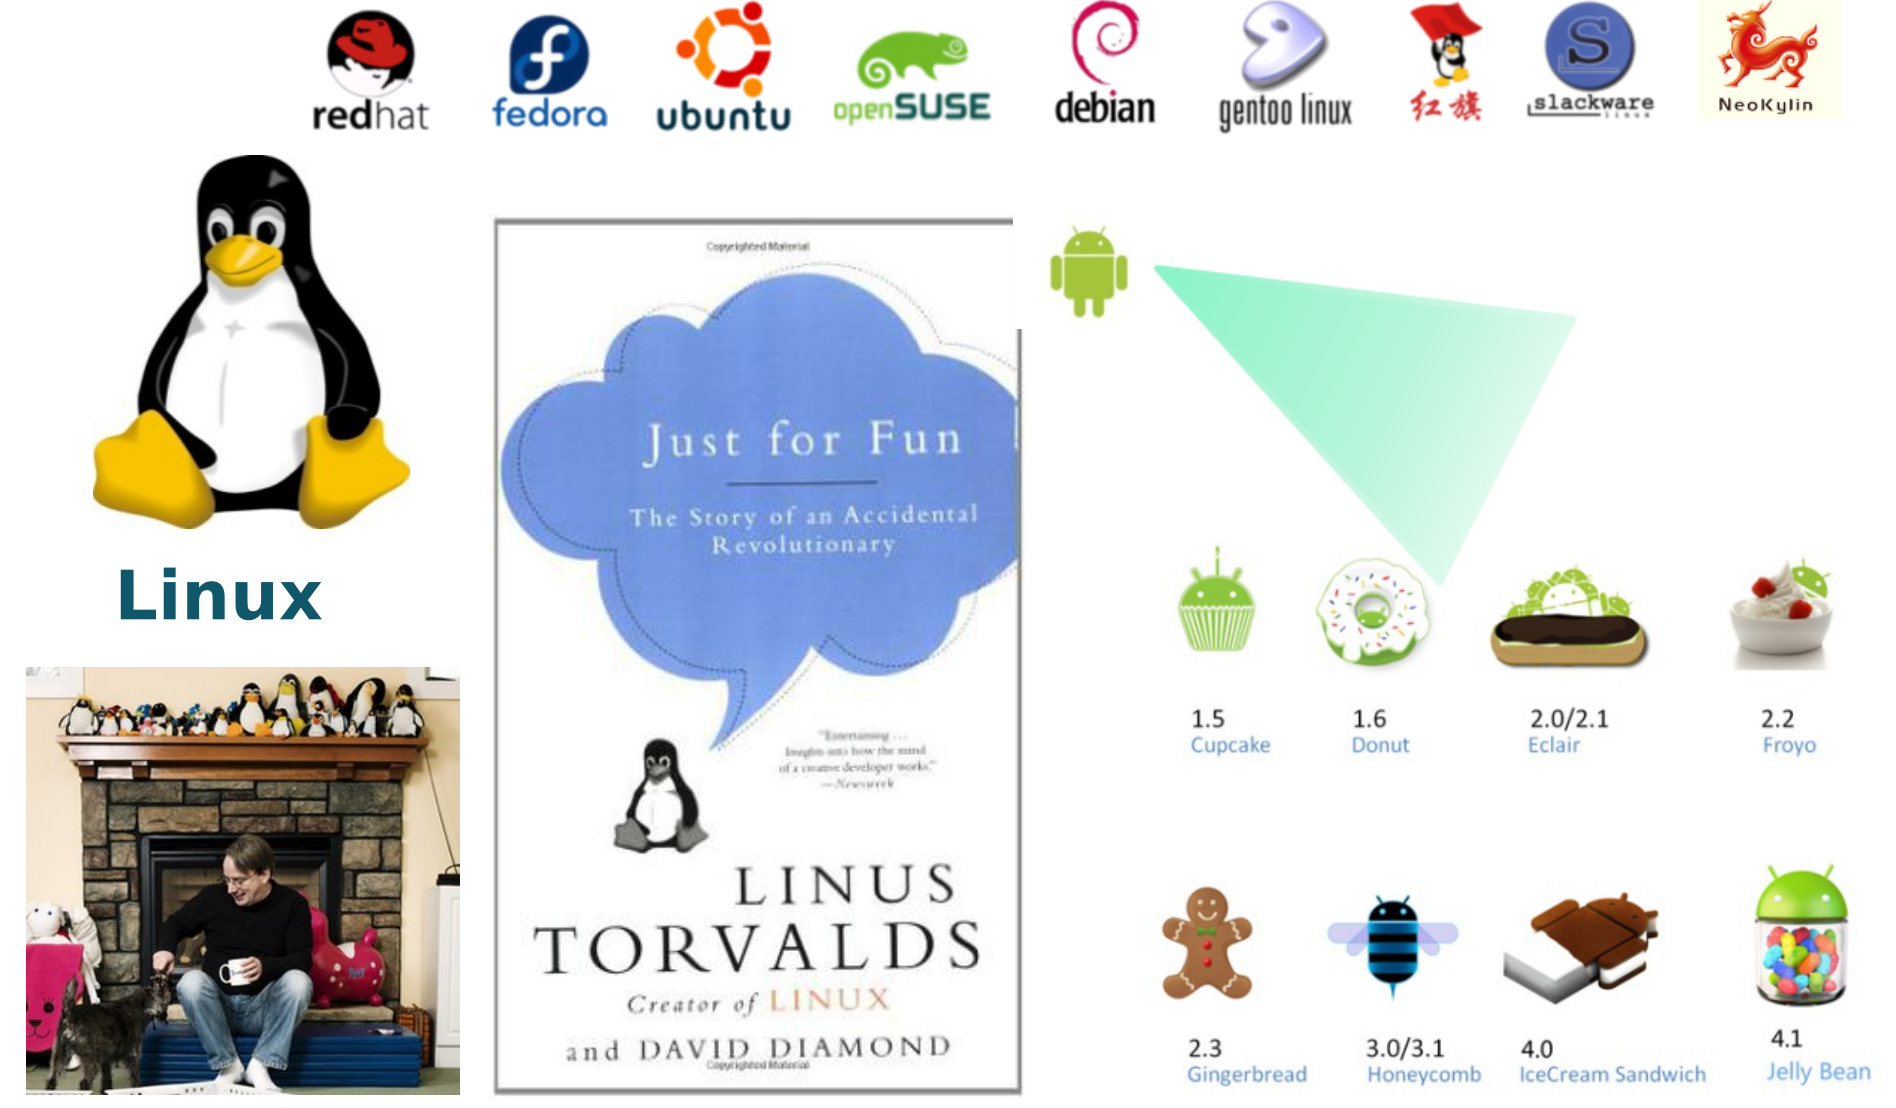
\includegraphics[width=1\linewidth]{linux-family}	
   \end{column}
 	
    \begin{column}{0.5\textwidth}
    \begin{itemize}
    \item 动机
    \begin{itemize}
    \item 已有操作系统很好,我将来的工作不会写操作系统
    \begin{itemize}
        \item Windows,Linux.android,ios
    \end{itemize}\pause
    \item 已有操作系统是否解决了所有的事?
        \begin{itemize}
        \item multi-core/parallel
        \item Non-Volatile Storage
        \item security
        \item Energy
        \item mobility/AIoT
        \item correct/verification
    \end{itemize}\pause
    \item \textit{为什么我要学习它?}
        \end{itemize}
    \end{itemize}
     \end{column}

     
%    \begin{column}{0.5\textwidth}
%    
%    \end{column}
    
    \end{columns}
    
    \end{frame}
%------------------------------------------------

%\begin{frame}
%    \frametitle{学习操作系统的目的}
%    \begin{columns}[t]
%    \begin{column}{0.5\textwidth}
%    \begin{itemize}
%    \item 动机
%    \begin{itemize}
%    \item 已有操作系统很好,我将来的工作不会写操作系统
%    \begin{itemize}
%        \item Windows,Linux.android,ios
%    \end{itemize}
%    \item 已有操作系统是否解决了所有的事?
%        \begin{itemize}
%        \item multi-core/parallel
%        \item Non-Volatile Storage
%        \item security
%        \item Energy
%        \item mobility/AIoT
%        \item correct/verification
%        \end{itemize}
%    \item 为什么我要学习它?
%       \end{itemize}
%    \end{itemize}
%     \end{column}
%     
%    \begin{column}{0.5\textwidth}
%        \begin{itemize}
%            \item 收获
%        \begin{itemize}
%            \item 操作系统很有用!
%                \begin{itemize}
%                    \item 掌握OS的基本原理
%                \end{itemize}
%            \item 我想了解操作系统到底是如何工作的?
%                \begin{itemize}
%                    \item 掌握OS机制的实现技术
%                \end{itemize}
%            \item 写操作系统很酷!
%                \begin{itemize}
%                    \item 经历开发一个OS的主要阶段
%                \end{itemize}
%            \item 掌握操作系统是一个挑战!
%                \begin{itemize}
%                    \item 加深对计算机系统的理解
%                \end{itemize}
%            \item 我要参与系统软件开发
%                \begin{itemize}
%                    \item 会将所学知识灵活应用
%                \end{itemize}
%            \end{itemize}
%        \end{itemize}
%        \end{column}
%    \end{columns}
%    
%    \end{frame}

%------------------------------------------------
    
\begin{frame}
    \frametitle{掌握操作系统具有挑战性(1)}
    
    \begin{columns}
    	
    \begin{column}{0.3\textwidth}	
      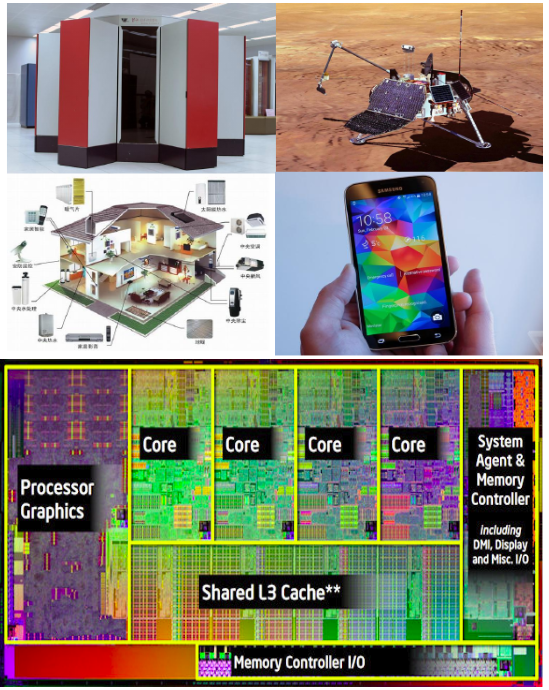
\includegraphics[width=1\linewidth]{os-challenge}	
    \end{column}

	\begin{column}{0.7\textwidth}
    
    \textbf{抓住操作系统的关键问题}
    \begin{itemize}
        \item 操作系统提供的抽象
            \begin{itemize}
                \item Win/Linux都有千万行代码,但都提供了很好的抽象
            \end{itemize} \pause
        \item 操作系统管理并发事务
            \begin{itemize}
                \item 并发导致有趣的编程挑战
            \end{itemize} \pause
        \item 操作系统代码保证对原始硬件的安全访问
            \begin{itemize}
               \item CPU、内存、磁盘
                \item 时间依赖行为, 非法行为, 硬件故障
            \end{itemize} \pause
        \item 操作系统代码理解和满足应用需求 \pause
%        \item 操作系统是系统安全的基础
            \begin{itemize}
            	\item 操作系统要及时地给应用提供合理资源
                \item 操作系统出错,就意味着机器出错,应用无法使用
                \item 操作系统必须比用户程序拥有更高的稳定性
            \end{itemize}
        
    \end{itemize}
    \end{column}

    \end{columns}

\end{frame}

%------------------------------------------------
    
\begin{frame}
    \frametitle{掌握操作系统具有挑战性(2)}
    
        \begin{columns}
    	
    	\begin{column}{0.3\textwidth}	
    		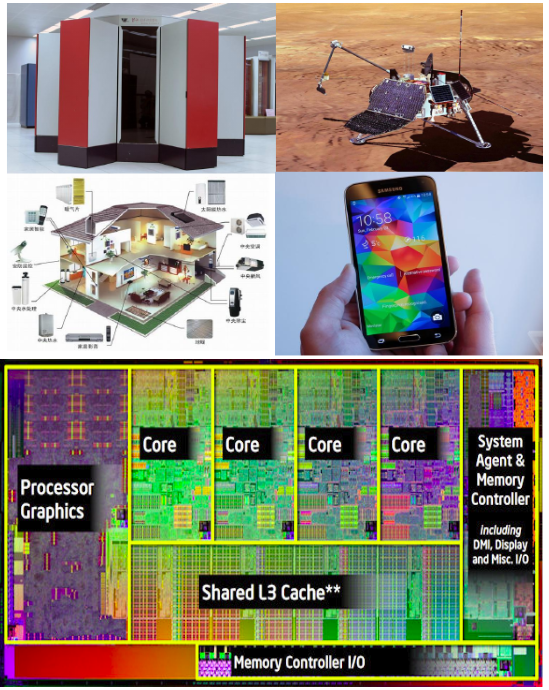
\includegraphics[width=1\linewidth]{os-challenge}	
    	\end{column}
    
    	\begin{column}{0.7\textwidth}
    		
     \textbf{理解操作系统需要具有系统思维} 
    \begin{itemize}
        \item 操作系统并不仅仅是一系列琐碎的算法
            \begin{itemize}
                \item 磁盘调度算法大多已被硬件实现
                \item 进程调度算法/页面置换算法等只是其中的一小部分
            \end{itemize} \pause
        \item 并发处理很关键,但只是是操作系统的一小部分
            \begin{itemize}
                \item 内核里不存在管程和哲学家问题
            \end{itemize} \pause
    \end{itemize}

    \begin{itemize}
	\item 建立联系
    \begin{itemize}
        \item 不同组成部分的相互关系?如何形成的整体?
    \end{itemize} \pause                
	\item 权衡资源
	\begin{itemize}
		\item 时间与空间 --性能的可预测性与公平性
	\end{itemize} \pause
	\item 软硬协同
	\begin{itemize}
		\item 如何让中断、异常、上下文切换真正有效? 
		\item TLB是如何工作的?这对页表又意味着什么?
	\end{itemize}
\end{itemize}

    \end{column}

\end{columns}

\end{frame}

%------------------------------------------------
%    
%\begin{frame}
%    \frametitle{掌握操作系统具有挑战性(3)}
%    \textbf{学习操作系统需要具有系统思维} \pause
%
%    \begin{itemize}
%        \item 权衡
%            \begin{itemize}
%                \item 时间与空间
%                \item 性能与可预测性
%                \item 公平与性能(哪种设计能工作?为什么?)
%            \end{itemize} \pause
%        \item 软硬协同
%            \begin{itemize}
%                \item 如何让中断、异常、上下文切换真正有效? 
%                \item TLB是如何工作的?这对页表又意味着什么?
%                \item 如果你不展示任何汇编代码,那么你就不是教操作系统的!
%            \end{itemize}
%    \end{itemize}
%\end{frame}

%------------------------------------------------
    
\begin{frame}
    \frametitle{如何上好操作系统这门课?}
\begin{block}{《儒效篇》--荀子}
不闻不若闻之,闻之不若见之,见之不若知之,
知之不若行之;学至于行之而止矣。 
\end{block} \pause     
\begin{block}{Thomas Edison }
   天才是1\%的灵感加上99\%的汗水 
\end{block} \pause
\begin{block}{往届同学}
   “最有趣的三年级课程!”  “最无聊的三年级课程!” “难过的三年级课程!”
\end{block}    

\end{frame}

%----------------------------------------------------------------------------------------

\end{document}
